\chapter{具有物理标度的结构与密度绘图}
\section{位移椭球的概率含义}
若原子位移为 $\vct u\sim\mathcal N(\vct0,\mat U)$，则 Mahalanobis 距离
\begin{equation}
q=\vct u^{\mathsf T}\mat U^{-1}\vct u
\end{equation}
服从三个自由度的 $\chi^2$ 分布。概率为 $p$ 的椭球边界满足
\begin{equation}
\vct u^{\mathsf T}\mat U^{-1}\vct u=\chi^2_3(p).
\end{equation}
令 $\mat U=\mat Q\diag(\lambda_1,\lambda_2,\lambda_3)\mat Q^{\mathsf T}$，则椭球主轴为 $\mat Q$ 的列，半轴为
\begin{equation}
a_i=\sqrt{\chi^2_3(p)\lambda_i}.
\label{eq:ellipsoid}
\end{equation}
绘制所谓“50\% 椭球”时，不能只用 $\sqrt{\lambda_i}$：三维总体概率与一维一个标准差不同。软件按式~\eqref{eq:ellipsoid} 生成表面，并用全部网格顶点的 Mahalanobis 距离检验实现。

\begin{figure}[htbp]
\centering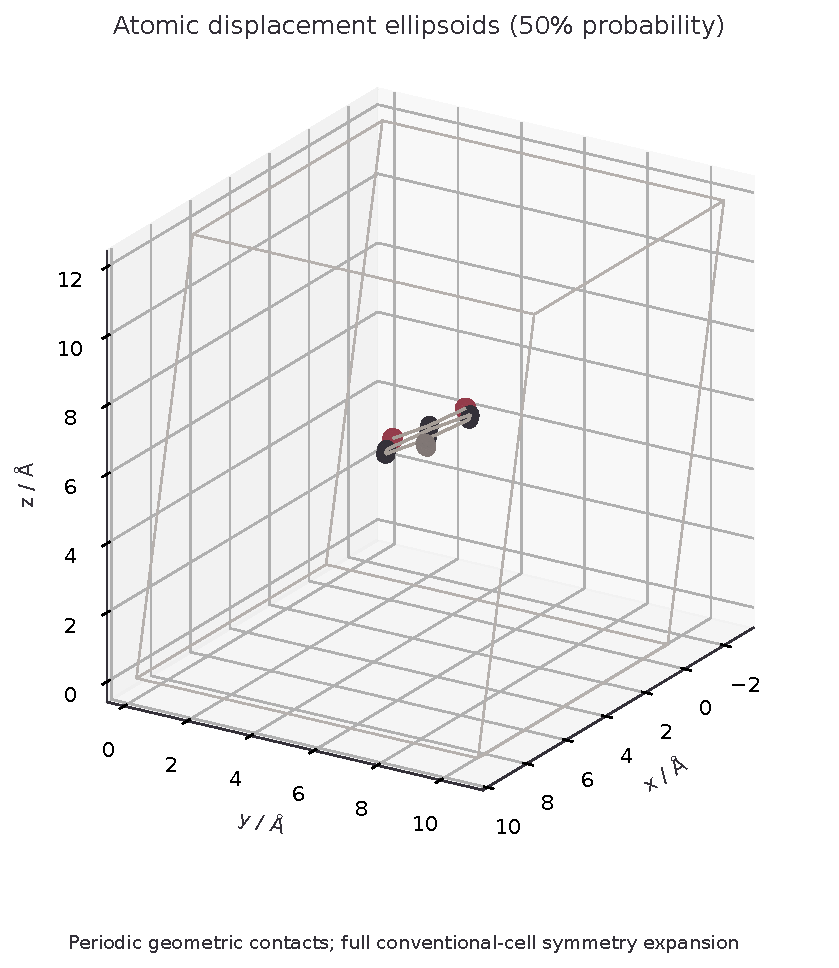
\includegraphics[width=.78\textwidth]{figures/structure_ellipsoids.pdf}
\caption{含各向异性 Br 位点的合成示例之 50\% 位移椭球。晶胞按真实非正交矩阵绘制；图中连接按元素半径与距离生成几何接触候选，不代表独立的化学键价判定。该图对应附录中的有噪声示例，并非实验结构。}
\end{figure}

\section{CIF 张量到笛卡尔张量}
CIF 与 SHELX 常将位移指数写作~\cite{cif_u}
\begin{equation}
T_h=\exp\left[-2\pi^2h^{\mathsf T}\mat D\mat U_{\mathrm{CIF}}\mat D h\right],
\qquad \mat D=\diag(|a^*|,|b^*|,|c^*|).
\end{equation}
因为 $\vct g=\mat A^{-\mathsf T}h$，与式~\eqref{eq:dw} 比较可得
\begin{equation}
\mat U_{\mathrm{cart}}=\mat A\mat D\mat U_{\mathrm{CIF}}\mat D\mat A^{\mathsf T}.
\label{eq:ucif}
\end{equation}
在斜晶胞中，直接把文件中的 $U_{ij}$ 当作笛卡尔协方差来画椭球，会同时改变方向和大小。实现通过不同反射的二次型保持不变来验证式~\eqref{eq:ucif}。

\section{常规差值电子密度}
给定精修模型和强度尺度 $k$，定义显示用幅度
\begin{equation}
F_{o,h}=\sqrt{\max(y_h/k,0)},\qquad
u_h=\begin{cases}F_{c,h}/|F_{c,h}|,&|F_{c,h}|>0,\\1,&|F_{c,h}|=0.\end{cases}
\end{equation}
常规无权重差值图与 $2F_o-F_c$ 图的系数为
\begin{equation}
C_h^{\Delta}=(F_{o,h}-|F_{c,h}|)u_h,
\qquad
C_h^{2o-c}=(2F_{o,h}-|F_{c,h}|)u_h.
\end{equation}
这些图使用模型相位，因此会带有相位偏倚。它们不是模型独立的密度测量，也不是含 $m$、$D$ 或 $\sigma_A$ 权重的统计最优地图。零级系数未知时取零会使显示图的平均密度为零；这一选择影响基线，不改变非零频率提供的结构信息。

精修使用的异常散射复系数一般不严格满足实密度的 Hermitian 条件。为生成实标量图，显示模块平均 $C_h$ 与 $C_{-h}^*$。这一处理仅用于地图，不合并或更改精修中的 Friedel 强度。完全重叠孪晶的观测强度也不属于单一振幅，因而默认不由其平方根直接生成差值密度；需要先有经过验证的去孪晶方案。

\section{从网格到等值面}
三维网格存储分数坐标采样。等值面算法在网格坐标中寻找与给定密度阈值的交点，再将网格位置 $\vct n$ 转为
\begin{equation}
\vct x=\diag(N_1^{-1},N_2^{-1},N_3^{-1})\vct n,
\qquad \vct r=\mat A\vct x.
\end{equation}
对斜晶胞，$\mat A$ 包含剪切和轴间夹角，不能用三个独立的轴长度相乘代替。实现为周期面追加首层切片，再作 marching cubes；追加切片之后，分母仍使用原始 $N_i$，否则整个晶胞会被人为收缩。

\begin{figure}[htbp]
\centering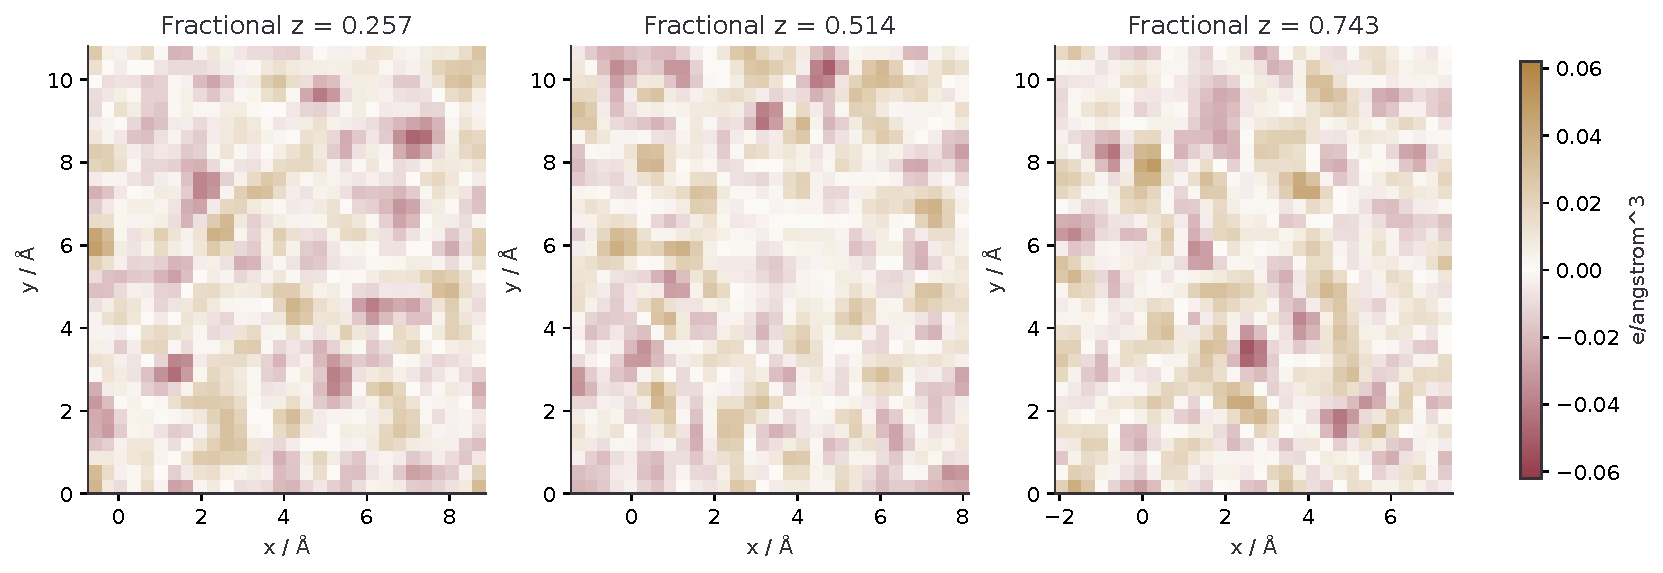
\includegraphics[width=\textwidth]{figures/density_sections.pdf}
\caption{合成示例的差值密度切片。色条给出实际密度单位；默认地图仅使用工作反射。切片和等值面不修改原始观测，缺失系数在显示地图中为零。}
\end{figure}

\section{倒易空间与统计诊断}
倒易空间点应画在 $\vct g_h=\mat B h$，而不是直接把 $h,k,l$ 当作欧氏坐标。颜色可编码标准化残差
\begin{equation}
z_h=\frac{y_h-\mu_h}{\sigma_h}.
\end{equation}
它能显示异常是否集中在特定倒易方向、分辨率范围或反射组。异常点只是需检查的候选，绘图不会自动删除它们。

\begin{figure}[htbp]
\centering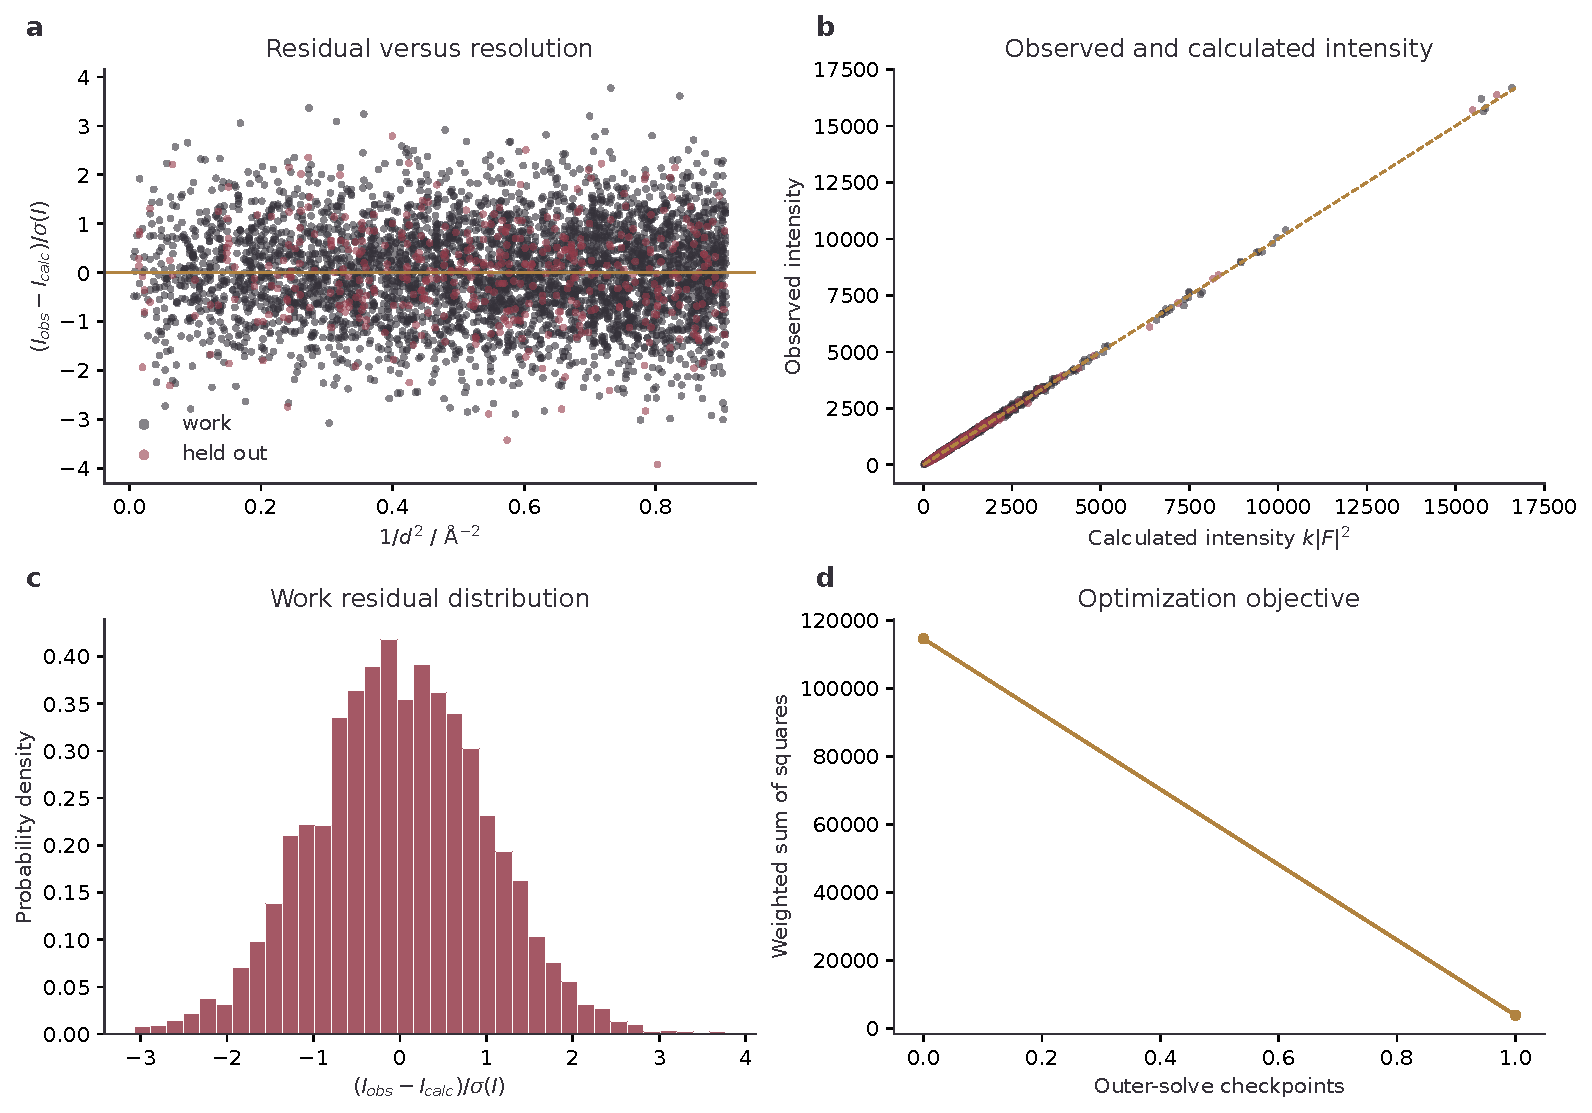
\includegraphics[width=\textwidth]{figures/refinement_diagnostics.pdf}
\caption{有噪声合成示例的强度一致性、分辨率依赖、残差分布及求解检查点。检查点记录初始状态和外层权重求解结束状态，并非每一次内部信赖域迭代。}
\end{figure}

参数相关图采用
\begin{equation}
R_{ij}=\frac{C_{ij}}{\sqrt{C_{ii}C_{jj}}}.
\end{equation}
它反映当前独立参数化下的局部相关。对 Cholesky 或 logit 变量，应结合参数名解释，不能将其直接称为原子笛卡尔坐标之间的相关图。秩亏时不绘制一个由伪逆伪装成的完整参数相关矩阵。

\section{交互图与可发表输出}
交互 HTML 在一个文件中嵌入绘图库，可离线旋转结构、查看原子属性、检查 Miller 指数与密度表面。静态输出采用 SVG 和 PDF 矢量格式，用于报告和论文排版。两者由相同的坐标、张量和数值结果生成，避免交互界面与最终图稿使用不同的科学数据。

绘图的可读性以明确信息为目标：椭球标明概率，地图标明类型和单位，反射图保留指数，合成数据标明来源。更多颜色和表面并不会增加证据；一张图应明确回答一个结构或模型诊断问题。
